\section*{Learning Objectives}

\begin{itemize}
\item Equations that have special structure are often much easier to solve
\item Some examples to show this.
\end{itemize}

\section*{Outcomes}
\begin{itemize}
\item Recognize triangular systems of linear equations and distinguish those with a unique answer.
\item Learn that the determinant of a square triangular matrix is the product of the terms on its diagonal.
    \item How to use forward and back substitution.
    \item Swapping rows of equations and permutation matrices.
\end{itemize}
\newpage

\section{Background}

\begin{itemize}
    \item A system of linear equations is \textbf{square} if it has the same number of equations as unknowns.
    
    \item If the system of linear equations is expressed in the form $Ax=b$, then it is \textbf{square} if, and only if, $A$ has the same number of rows as it has columns; that is, $A$ is $ n \times n$.
    
\item A square system of linear equations 
    $Ax=b,$
    has a \textbf{unique solution} $x$ for any $n\times 1$ vector $b$ if, and only if, the $n \times n$ matrix $A$ satisfies $\det(A) \neq 0.$

    \item Computing the \textbf{determinant} of a general square matrix is tedious.  
    
    \item The \textbf{diagonal} of the square matrix $$A=\left[\begin{array}{cccc} \RED a_{11} & a_{12} & \cdots & a_{1n}\\
a_{21} & \RED a_{22} & \cdots & a_{2n} \\ \vdots & \vdots & \RED \ddots& \vdots \\
a_{n1} & a_{n2} & \cdots & \RED a_{nn}\\\end{array}\right]$$
is 
$$ {\rm diag}(A)=\begin{bmatrix}a_{11} & a_{22} & \ldots & a_{nn} \end{bmatrix}. $$
The diagonal consists of all elements $a_{ij}$ of $A$ such that $j=i$.

\item The elements of $A$ that are \textbf{not on the diagonal} are called the \textbf{off-diagonal elements}.

\end{itemize}

\section{A Warm-up with Diagonal Systems of Linear Equations}

As a warm-up to the main topic, we want to illustrate that some systems of linear equations are easy to solve, independently of the number of unknowns. We'll start small, and then go big!\\

This is an example of a square system of linear equations that is \textit{Diagonal},
\begin{equation}
    \begin{aligned}
     4 x_1 &=6 \\
      - x_2 &= 7\\
 3 x_3  &= 2.
    \end{aligned}
\end{equation}
Computing the solution of the set of diagonal equations is trivial because we just have to divide each row of the equation by the element multiplying the unknown, namely
\begin{equation}
\label{eq:Diag00}
    \begin{aligned}
     4 x_1 &=6 \\
      - x_2 &= 7\\
 3 x_3  &= 2.
    \end{aligned} \iff     \begin{aligned}
    x_1 &=\frac{6}{4} = \frac{3}{2}\\
      x_2 &= \frac{7}{-1} = -7\\
 x_3  &= \frac{2}{3}.
    \end{aligned} 
\end{equation}
In this example, all of the constants multiplying the unknowns were non-zero. If one of them had been zero, for example, if the second row were $0 x_2 = 7$, then the equations would not have a solution; if the second row were $0 x_2 = 0$, then the equations would have an infinite number of solutions because $x_2$ could take on any value.\\

When we write the system as $Ax=b$, we have
\begin{equation} 
\label{eq:Diag01}
\begin{aligned}
     4 x_1 &=6 \\
      - x_2 &= 7\\
 3 x_3  &= 2.
    \end{aligned}\iff \underbrace{\left[\begin{array}{rrr} 4 & \RED 0 & \RED 0\\
\RED 0 & -1 & \RED 0 \\ \RED 0 &\RED 0 & 3  \end{array}\right]}_{A}  \underbrace{\left[\begin{array}{c} x_1 \\x_2 \\x_3\end{array} \right]}_{x}
= \underbrace{\left[\begin{array}{r} 6 \\7 \\2\end{array} \right]}_{b}.
\end{equation}
where we note that all of the \textcolor{red}{off-diagonal terms} of the matrix $A$ are zero. More precisely, the condition is 
 $a_{ij}=0$ for all $i \neq j$. Such matrices are called \textit{Diagonal Matrices}. \\
 
 The corresponding system of linear equations is easy to solve because each of the coefficients $a_{11}=4$, $a_{22}=-1$, and $a_{33}=3$  multiplying the unknowns $x_1$, $x_2$, and $x_3$ is non-zero. For later use, we note that $n$ real numbers  $a_{11}$, $a_{22}$, ..., $a_{nn}$ are all non-zero if, and only if, their product is non-zero, that is,  
 $$ a_{11}\neq 0, a_{22} \neq 0, \ldots, a_{nn} \neq 0 \iff  a_{11} a_{22} \cdots  a_{nn} \neq 0.$$
This result is true because the product of any two real numbers is zero if, and only if, at least one of the numbers is zero.\\

More generally, a square $n \times n$ matrix $A$ where all of the \textbf{off-diagonal} elements are zero is said to be a \textbf{diagonal matrix},
    $$A=\left[\begin{array}{cccc} \BLUE a_{11} & \RED 0 & \cdots & \RED 0\\
\RED 0& \BLUE a_{22} & \cdots & \RED 0 \\ \RED \vdots & \RED \vdots & \BLUE \ddots& \RED \vdots \\
\RED 0 & \RED 0 & \cdots & \BLUE a_{nn}\\\end{array}\right];$$
in other words, if $a_{ij}=0$ for all $i \neq j$, then $A$ is diagonal. Computing the \textbf{determinant} of a diagonal matrix is very easy, 
$$\det(A) = \left|\begin{array}{cccc} \BLUE a_{11} & \RED 0 & \cdots & \RED 0\\
\RED 0& \BLUE a_{22} & \cdots & \RED 0 \\ \RED \vdots & \RED \vdots & \BLUE \ddots& \RED \vdots \\
\RED 0 & \RED 0 & \cdots & \BLUE a_{nn}\\\end{array}\right| = a_{11} a_{22} \cdots a_{nn},$$
the product of the terms on its diagonal.\\

A diagonal system of $n$ linear equations 
\begin{equation} 
\label{eq:Diag02}
\begin{aligned}
     a_{11} x_1 &=b_1\\
      a_{22}x_2 &= b_2\\
      \vdots~~~~ &=   ~    \vdots \\
 a_{nn} x_n  &= b_n
    \end{aligned}\iff \underbrace{\left[\begin{array}{cccc} \BLUE a_{11} & \RED 0 & \cdots & \RED 0\\
\RED 0& \BLUE a_{22} & \cdots & \RED 0 \\ \RED \vdots & \RED \vdots & \BLUE \ddots& \RED \vdots \\
\RED 0 & \RED 0 & \cdots & \BLUE a_{nn}\\\end{array}\right]}_{A}  \underbrace{\left[\begin{array}{c} x_1 \\x_2 \\ \vdots\\x_n\end{array} \right]}_{x}
= \underbrace{\left[\begin{array}{r} b_1 \\b_2 \\ \vdots \\b_n\end{array} \right]}_{b}
\end{equation}
is straightforward to solve, no matter its size, because, whenever $a_{ii} \neq 0$, we have 
\begin{equation}
\label{eq:Diag03}
    x_i = \frac{b_i}{a_{ii}}.
\end{equation}
If one of the coefficients $a_{ii}$ on the diagonal is zero, then, if the corresponding element $b_i$ is non-zero, we deduce that the equations do not have a solution, and if the corresponding element $b_i$ is zero, we deduce that the equations can have an infinite number of solutions. This is identical to the discussion below \eqref{eq:Diag00}. \\

For diagonal matrices, it follows that if $\det(A) \neq 0$, then $Ax=b$ has a unique solution; moreover the solution is very easy to compute via \eqref{eq:Diag03}. In the next Section, we explore other types of matrices that make computing a solution very fast and easy.

\section{Lower Triangular Systems of Linear Equations}

This is an example of a square system of linear equations that is \textit{Lower Triangular}
\begin{equation}
    \begin{aligned}
     3 x_1 &=6 \\
     2 x_1 - x_2 &= -2\\
    x_1 - 2 x_2 + 3 x_3  &= 2.
    \end{aligned}
\end{equation}

When we write the system as $Ax=b$, in the lower triangular case we have
\begin{equation} 
\label{eq:LT01}
\begin{aligned}
     3 x_1 &=6 \\
     2 x_1 - x_2 &= -2\\
    x_1 - 2 x_2 + 3 x_3  &= 2
    \end{aligned} \iff \underbrace{\left[\begin{array}{rrr} 3 & \RED 0 & \RED 0\\
2 & -1 & \RED 0 \\ 1 & -2 & 3  \end{array}\right]}_{A}  \underbrace{\left[\begin{array}{c} x_1 \\x_2 \\x_3\end{array} \right]}_{x}
= \underbrace{\left[\begin{array}{r} 6 \\-2 \\2\end{array} \right]}_{b}.
\end{equation}
where we note that all terms ``above'' the diagonal of the matrix $A$ are zero. More precisely, the condition is 
 $a_{ij}=0$ for all $j > i$. Such matrices are called \textit{lower-triangular}. \\


Here are two more examples of square lower triangular systems
\begin{equation}
\label{eq:LT02}
\begin{array}{cc}
  \begin{aligned}
     3 x_1 &=6 \\
     2 x_1 - x_2 & =0
    \end{aligned} &  \iff \underbrace{\left[\begin{array}{rr} 3 & \RED 0\\
2 & -1  \end{array}\right]}_{A}  \underbrace{\left[\begin{array}{c} x_1 \\x_2 \end{array} \right]}_{x}
= \underbrace{\left[\begin{array}{r} 6 \\0 \end{array} \right]}_{b}
    \end{array}
\end{equation}

\begin{equation}
\label{eq:LT03}
\begin{array}{cc}
   \begin{aligned}
     3 x_1 &=6 \\
     2 x_2 &= -2\\
    x_1 - 2 x_2 &= 2 \\
    x_1 - x_3 + 2 x_4 &= 10
    \end{aligned} \iff \underbrace{\left[\begin{array}{rrrr} 3 & \RED 0 & \RED 0 & \RED 0\\
0 & 2 & \RED 0 & \RED 0\\ 1 & -2& 0 & \RED 0 \\ 1 & 0 & -1 & 2  \end{array}\right]}_{A}  \underbrace{\left[\begin{array}{c} x_1 \\x_2 \\x_3 \\x_4\end{array} \right]}_{x}
= \underbrace{\left[\begin{array}{r} 6 \\-2 \\2 \\10\end{array} \right]}_{b}
    \end{array}
\end{equation}


The following systems of linear equations are square, but they are not lower triangular. The ``offending term'' is boxed,
\begin{equation}
\label{eq:notLT01}
\begin{array}{cc}
    \begin{aligned}
     3 x_1 &=6 \\
     2 x_1 - x_2 -\boxed{x_3} &= -2\\
    x_1 - 2 x_2 + 3 x_3  &= 2
    \end{aligned} &  \iff \underbrace{\left[\begin{array}{rrc} 3 & 0 & 0\\
2 & -1 & \boxed{-1} \\ 1 & -2 & 3  \end{array}\right]}_{A}  \underbrace{\left[\begin{array}{c} x_1 \\x_2 \\x_3\end{array} \right]}_{x}
= \underbrace{\left[\begin{array}{r} 6 \\-2 \\2\end{array} \right]}_{b}
    \end{array}
\end{equation}
and
\begin{equation}
\label{eq:notLT02}
\begin{array}{cc}
  \begin{aligned}
     3 x_1 + \boxed{3 x_2} &=6 \\
     2 x_1 - 2 x_2&= 0
    \end{aligned} &  \iff \underbrace{\left[\begin{array}{rc} 3 & \boxed{3}\\
2 & -1  \end{array}\right]}_{A}  \underbrace{\left[\begin{array}{c} x_1 \\x_2 \end{array} \right]}_{x}
= \underbrace{\left[\begin{array}{r} 6 \\0 \end{array} \right]}_{b}
    \end{array}
\end{equation}

\begin{tcolorbox}[sharp corners, colback=green!30, colframe=green!80!blue, title=\textbf{\large Triangular Matrices}]
The key ingredients of a square lower triangular system are 
\begin{itemize}
    \item The unknowns are ordered, as in $\begin{pmatrix} x_1 & x_2 & \ldots&  x_n \end{pmatrix}$ or $\begin{pmatrix} u & v & w & x & y & z \end{pmatrix}$
    \item The first equation only involves the first unknown.
    \item The second equation involves only the first two unknowns
    \item More generally, the $i$-th equation involves only the first $i$ unknowns.
    \item The coefficients $a_{ij}$ on or below the diagonal can be zero or non-zero. 
\end{itemize}
\end{tcolorbox}

From a matrix point of view, the condition is, all terms above the diagonal are zero. What does this mean? It means that $A$ looks like this, 
\begin{equation}
\label{eq:BigALowerTriangular}
A=\left[\begin{array}{ccccccc} {\bf a_{11}} & \RED  0&  \RED 0 & \RED 0 & \RED \cdots & \RED 0 &\RED 0 \medskip\\
a_{21} & {\bf a_{22}} & \RED 0 & \RED 0 & \RED \cdots & \RED 0 & \RED 0  \medskip\\ 
a_{31} & a_{32} & {\bf a_{33}} & \RED 0 & \RED \cdots & \RED 0 &   \medskip \RED 0\\
\vdots & \vdots & \vdots & {\boldsymbol \ddots}  & \RED\ddots &\RED 0 & \RED 0  \medskip\\
\\
\vdots & \vdots & \vdots & \vdots &  {\boldsymbol \ddots} &   \RED 0 & \RED 0  \medskip\\
a_{(n-1)1} & a_{(n-1)2} & a_{(n-1)3} & a_{(n-1)4} & \cdots & {\bf a_{(n-1)(n-1)} } & \RED 0 \medskip \\
a_{n1} & a_{n2} & a_{n3} & a_{n4} & \cdots & a_{n(n-1)} & {\bf a_{nn} } \end{array}\right],
\end{equation}
namely, $a_{ij} = 0$ for $j > i$. Note that the diagonal is in bold and the terms above the diagonal are in red. The matrices in \eqref{eq:LT01} through \eqref{eq:LT03} are \textit{lower triangular}, while the matrices in \eqref{eq:notLT01} and 
\eqref{eq:notLT02} are not lower triangular.

\section{Determinant of a Lower Triangular Matrix}

\begin{tcolorbox}
\textbf{Highly Useful Fact:} The matrix determinant of a square lower triangular matrix is equal to the product of the elements on the diagonal. For the matrix $A$ in \eqref{eq:BigALowerTriangular}, its determinant is 
\begin{equation}
   \det(A) = a_{11} \cdot a_{22} \cdot \ldots \cdot a_{nn}. 
\end{equation}
\end{tcolorbox}

Hence, for lower triangular matrices of size $10 \times 10$ or so, the determinant can be computed by inspection! Let's do a few:
$$\det\left( \left[\begin{array}{rrr} 3 & 0 & 0\\
2 & -1 & 0 \\ 1 & -2 & 3  \end{array}\right] \right) = 3 \cdot (-1) 3 = -9 \neq 0.$$
Hence, the system of equations \eqref{eq:LT01} has a unique solution.\\

Let's now use the alternative notation for the determinant of a matrix, 
$$ \left|\begin{array}{rrrr} 3 & 0 & 0 & 0\\
0 & 2 & 0 & 0\\ 1 & -2& 0 &0 \\ 1 & 0 & -1 & 2  \end{array}\right| = 3\cdot 2\cdot 0 \cdot 2 = 0.  $$
Hence, the system of equations \eqref{eq:LT03} is one of the problem cases: it may have no solution or it may have an infinite number of solutions.\\

\begin{tcolorbox}
\textbf{Remark:} For a square lower triangular matrix, the matrix determinant is nonzero if, and only if, all of the elements on the diagonal of the matrix are non-zero. Equivalently, for a square lower triangular matrix, the matrix determinant is zero if, and only if, at least one of the elements on the diagonal of the matrix is zero. In other words, we do not really need to multiply them out to check for $\det(A) \neq 0$, the condition for uniqueness of solutions of square systems of linear equations.
\end{tcolorbox}

\section{Lower Triangular Systems and Forward Substitution}
\label{sec:ForwardSubstitution}

We develop a solution to a lower triangular system by starting at the top and working our way to the bottom via a method called \textbf{forward substitution}. As an example, we use \eqref{eq:LT01}, which for convenience, we repeat here:
\begin{equation} 
\label{eq:LT01b}
\begin{aligned}
     3 x_1 &=6 \\
     2 x_1 - x_2 &= -2\\
    x_1 - 2 x_2 + 3 x_3  &= 2
    \end{aligned} \iff \underbrace{\left[\begin{array}{rrr} 3 & \RED 0 & \RED 0\\
2 & -1 & \RED 0 \\ 1 & -2 & 3  \end{array}\right]}_{A}  \underbrace{\left[\begin{array}{c} x_1 \\x_2 \\x_3\end{array} \right]}_{x}
= \underbrace{\left[\begin{array}{r} 6 \\-2 \\2\end{array} \right]}_{b}.
\end{equation}

Because we have ordered the variables as $\begin{pmatrix} x_1 & x_2 &x_3\end{pmatrix}$, we isolate $x_1$ in the first equation, $x_2$ in the second equation, and $x_3$ in the third equation by moving the other variables to the right-hand side,
\begin{equation}
    \begin{aligned}
3 x_1 &= 6 \\
 -x_2 &= -2 -2 x_1 \\
  3 x_3  &= 2 -x_1 + 2 x_2 .
    \end{aligned}
\end{equation}
You can see how the first equation is trivial, and so is the second one, once the first is solved, etc. Next, we can make the coefficients of the leading variables  all equal to one by dividing through by the coefficients that multiply them, yielding
\begin{equation}
    \begin{aligned}
 x_1 &=\frac{1}{3} 6 = 2\\
 x_2 &= -\left[ -2 -2 x_1\right] = 2 + 2 x_1\\
  x_3  &=\frac{1}{3}\left[ 2 -x_1 + 2 x_2\right].
    \end{aligned}
\end{equation}
Next, we substitute in, working from top to bottom:
\begin{equation}
    \begin{aligned}
     x_1 &=\frac{1}{3} 6 = 2\\
 x_2 &=  2 + 2 x_1 = 6\\
     x_3  &=\frac{1}{3}\left[ 2 -x_1 + 2 x_2 \right]=\frac{1}{3}\left[12 \right] =  4,
    \end{aligned}
\end{equation}

\begin{tcolorbox}[sharp corners, colback=green!30, colframe=green!80!blue, title=\textbf{\Large Forward Substitution}]
The method is called \textbf{forward substitution} because once we have solved $x_1$, we take its value forward to the next equation where we solve for $x_2$, and once we have solved for $x_1$ and $x_2$, we take their values forward to the next equation where we solve for $x_3$. I am guessing that you see the pattern. \\

\textbf{When can forward substitution go wrong?} Well first of all, we only use it for lower triangular systems of linear equations. If the diagonal of the matrix corresponding to the system of linear equations has a zero on it, then the matrix determinant is zero ($\implies$ no solution or an infinite number of solutions) and forward substitution would lead us to \textbf{divide by zero, which we know is a major error in mathematics}. 
\end{tcolorbox}
As an example, we take \eqref{eq:LT03}, which we repeat here
\begin{equation}
\label{eq:LT03b}
\begin{array}{cc}
   \begin{aligned}
     3 x_1 &=6 \\
     2 x_2 &= -2\\
    x_1 - 2 x_2 &= 2 \\
    x_1 - x_3 + 2 x_4 &= 10.
    \end{aligned} \iff \underbrace{\left[\begin{array}{rrcr} 3 & 0 & 0 & 0\\
0 & 2 & 0 & 0\\ 1 & -2& \boxed{0} &0 \\ 1 & 0 & -1 & 2  \end{array}\right]}_{A}  \underbrace{\left[\begin{array}{c} x_1 \\x_2 \\x_3 \\x_4\end{array} \right]}_{x}
= \underbrace{\left[\begin{array}{r} 6 \\-2 \\2 \\10\end{array} \right]}_{b}
    \end{array}
\end{equation}
When we try to isolate $x_3$ in the third equation, we have a problem. To make it more obvious, we make $x_3$ explicit with its corresponding coefficient of zero
\begin{equation}
\begin{array}{ccc}
\left. \begin{aligned}
     3 x_1 &=6 \\
     2 x_2 &= -2\\
    x_1 - 2 x_2 + \boxed{ 0 x_3}&= 2 \\
    x_1 - x_3 + 2 x_4 &= 10 
    \end{aligned} \right\} & \left. \implies ~~
    \begin{aligned}
     3 x_1 &=6 \\
     2 x_2 &= -2\\
    \boxed{0 x_3}&= 2 -( x_1 - 2 x_2)\\
   2 x_4 &= 10 -( x_1 - x_3 )
    \end{aligned} \right\} \stackrel{\textbf{???}}{\implies}
    \begin{aligned}
    x_1 &=2 \\
     x_2 &= -1\\
x_3&= \boxed{\frac{1}{0}} \cdot (-2) ~~?!? ~\text{Divide by zero: not allowed!}\\
x_4 &= \frac{1}{4}(10 -2 + \frac{-2}{0})~~?!?!?~~\textbf{Wrong!}
    \end{aligned}
    \end{array}
 \end{equation}


\section{Upper Triangular Systems, Upper Triangular Matrices, Determinants, and Back Substitution}
\label{sec:BackSubstitution}
This is an example of a square \textbf{upper triangular system of equations} and its corresponding \textbf{upper triangular matrix}

\begin{equation} 
\label{eq:UT01b}
\begin{array}{cc}
    \begin{aligned}
     x_1 + 3x_2 + 2 x_3 &=6 \\
     2 x_2 +x_3 &= -2\\
     3 x_3 &= 4,
    \end{aligned} & \iff \underbrace{\left[\begin{array}{rrr} 
    1 & 3 & 2\\
\RED 0 & 2 & 1 \\ 
\RED 0 & \RED  0 & 3  \end{array}\right]}_{A}  
\underbrace{\left[\begin{array}{c} x_1 \\x_2 \\x_3\end{array} \right]}_{x}
= \underbrace{\left[\begin{array}{r} 6 \\-2 \\4\end{array} \right]}_{b}.
\end{array}
\end{equation}
We note that all of the coefficients of $A$ \textit{below the diagonal} are zero; that is $a_{ij}=0$ for $i > j$.\\

\begin{tcolorbox}
\textbf{Highly Useful Fact:} The matrix determinant of a square upper triangular matrix is equal to the product of the elements on the diagonal. For the matrix $A$ in \eqref{eq:UT01b}, its determinant is 
\begin{equation}
   \det(A) = 1 \cdot 2 \cdot 3 = 6. 
\end{equation}
Hence, we know the system of equations has a unique solution.
\end{tcolorbox}

\begin{tcolorbox}[sharp corners, colback=green!30, colframe=green!80!blue, title=\textbf{\Large Back Substitution}]
We develop a solution to an \textbf{upper triangular system of linear equations} by starting at the bottom and work our way to the top via \textbf{back substitution}. We first solve for the leading variables, which here we do in one step,
\begin{equation}
    \begin{aligned}
         x_1  &=6- (3x_2 + 2 x_3) \\
      x_2 &= \frac{1}{2} \left( -2-x_3 \right) \\
      x_3 &= \frac{4}{3},
    \end{aligned}
\end{equation}
but of course, you can do it in two steps as we did for lower triangular systems.
Next, we do back substitution, from bottom to top, sequentially plugging in numbers from the previous equations
\begin{equation}
    \begin{array}{llll}
         x_1  &=6- (3x_2 + 2 x_3) &= 6 -( 3\cdot(-\frac{5}{3}) + 2 \cdot \frac{4}{3}) &=\frac{18}{3}+\frac{7}{3} = \frac{25}{3}=8 \frac{1}{3} \medskip \\
        x_2 &= \frac{1}{2} \cdot \left( -2-x_3 \right) &=  \frac{1}{2} \cdot  \left( -2-\frac{4}{3} \right) &= \frac{1}{2} \cdot  \left(-\frac{10}{3}\right) = -\frac{5}{3} = -1 \frac{2}{3}\medskip \\
      x_3 &= \frac{4}{3}.
    \end{array}
\end{equation}
\end{tcolorbox}


\section{General Cases}

 The general form of a lower triangular system with a non-zero determinant is
\begin{equation}
    \begin{aligned}
         a_{11} x_1 &= b_1  ~~~(a_{11} \neq 0) \\
          a_{21} x_1 + a_{22} x_2 &=b_2 ~~~(a_{22} \neq 0)\\
     \vdots &= \vdots \\
          a_{n1} x_1 + a_{n2} x_2 + a_{n3} x_3+ \cdots +  a_{nn} x_n &=b_n ~~~(a_{nn} \neq 0)
    \end{aligned}
\end{equation}
and the solution proceeds from top to bottom, like this
\begin{equation}
    \begin{aligned}
         x_1 &= \frac{b_1}{a_{11}}  ~~~(a_{11} \neq 0) \\
           x_2 &= \frac{b_2- a_{21} x_1}{a_{22}} ~~~(a_{22} \neq 0)\\
     \vdots &= \vdots \\
          x_n &=\frac{b_n-a_{n1} x_1 - a_{n2} x_2 - \cdots  -a_{n,n-1} x_{n-1}}{a_{nn}}    ~~~(a_{nn} \neq 0).
    \end{aligned}
\end{equation}

The general form of an upper triangular system with a non-zero determinant is
\begin{equation}
\label{eq:GeneralUpperTriangular}
    \begin{aligned}
     a_{11} x_1 + a_{12} x_2 + a_{13} x_3+ \cdots +  a_{1n} x_n &=b_1 ~~~(a_{11} \neq 0)\\
     a_{22} x_2 + a_{23} x_3 + \cdots +  a_{2n} x_n &=b_2 ~~~(a_{22} \neq 0)\\
       a_{33} x_3 + \cdots +  a_{3n} x_n &=b_3 ~~~(a_{33} \neq 0)\\
     \vdots &= \vdots \\
%     a_{n-1,n-1} x_{n-1} +  a_{n-1,n} x_n &=b_{n-1} ~~~(a_{n-1,n-1} \neq 0)\\
     a_{nn} x_n &= b_n  ~~~(a_{nn} \neq 0),
    \end{aligned}
\end{equation}
and the solution proceeds from the \textbf{bottom} of \eqref{eq:GeneralUpperTriangular} to its \textbf{top}, like this,
% \begin{equation}
%     \begin{aligned}
%       x_1  &=\frac{b_1- a_{12} x_2 - \cdots -  a_{1n} x_n}{a_{11}} &(a_{11} \neq 0)\\
%      x_2 &= \frac{b_2-  a_{23} x_3 - \cdots -  a_{2n} x_n}{a_{22}} &(a_{22} \neq 0)\\
%     %   a_{33} x_3 + \cdots +  a_{3n} x_n &=b_3 ~~~(a_{33} \neq 0)\\
%   \vdots &= \vdots & \vdots~~~~~ \\
%       x_{n-1}  &= \frac{b_{n-1}- a_{n-1,n} x_n}{a_{n-1,n-1}}  &(a_{n-1,n-1} \neq 0)\\
%       x_n &= \frac{b_n}{a_{nn}}  &(a_{nn} \neq 0),
%     \end{aligned}
% \end{equation}
\begin{equation}
    \begin{aligned}
    x_n &= \frac{b_n}{a_{nn}}  &(a_{nn} \neq 0) \medskip \\
     x_{n-1}  &= \frac{b_{n-1}- a_{n-1,n} x_n}{a_{n-1,n-1}}  &(a_{n-1,n-1} \neq 0)\\
       \boldmath \vdots \unboldmath~~~ &=~~~~  \boldmath \vdots \unboldmath &  \boldmath \vdots \unboldmath~~~~~ \\
        x_2 &= \frac{b_2-  a_{23} x_3 - \cdots -  a_{2n} x_n}{a_{22}} &(a_{22} \neq 0)\\
      x_1  &=\frac{b_1- a_{12} x_2 - \cdots -  a_{1n} x_n}{a_{11}} &(a_{11} \neq 0)
    \end{aligned}
\end{equation}


\textbf{Remark:} For $1 \le i <n$, we need to form the product 
$$ a_{i,i+1}x_{i+1} + a_{i,i+2}x_{i+2} + \cdots + a_{i,n}x_{n}.$$
In Julia, there are two ways to do it
\begin{lstlisting}[language=Julia,style=mystyle]
method1 = A[i,i+1:n]'*x[i+1:n]
method2 = (A[i:i,i+1:n]*x[i+1:n])[1]
\end{lstlisting}
In method one, $A[i,i+1:n]$ is a column vector while $ A[i,i+1:n]'$ is a row vector. When it is multiplied by the column vector, $x[i+1:n]$, it produces a scalar. In method two, $A[i:i,i+1:n]$ is a $1 \times (n-i)$ matrix, which in Julia, is different than a row vector. When it is multiplied by the column  $x[i+1:n]$, it produces a $1 \times 1$ matrix. You then have to extract its value, which is done via $(A[i:i,i+1:n]*x[i+1:n])[1]$. See the ``tinyMatrix'' example in Lab \#1.\\

%\section{Matrix View of Triangular Systems of Equations}


% When we write the system as $Ax=b$, in the lower triangular case we have
% $$     \begin{aligned}
%      3 x_1 &=6 \\
%      2 x_1 - x_2 &= -2\\
%     x_1 - 2 x_2 + 3 x_3  &= 2
%     \end{aligned} \iff \underbrace{\left[\begin{array}{rrr} 3 & 0 & 0\\
% 2 & -1 & 0 \\ 1 & -2 & 3  \end{array}\right]}_{A}  \underbrace{\left[\begin{array}{c} x_1 \\x_2 \\x_3\end{array} \right]}_{x}
% = \underbrace{\left[\begin{array}{r} 6 \\-2 \\2\end{array} \right]}_{b}$$
% where we note that all terms ``above'' the diagonal of the matrix $A$ are zero. More precisely, the condition is 
%  $a_{ij}=0$ for all $j > i$. Such matrices are called lower-triangular. 
 
%  For the upper triangular case, we have 
% $$     \begin{aligned}
%      x_1 + 3x_2 + 2 x_3 &=6 \\
%      2 x_2 +x_3 &= -2\\
%      3 x_3 &= 4,
%     \end{aligned} \iff \underbrace{\left[\begin{array}{ccc} 1 & 3 & 2\\
% 0 & 2 & 1 \\ 0 & 0 & 3 \end{array}\right]}_{A} \underbrace{\left[\begin{array}{c} x_1 \\x_2 \\x_3\end{array} \right]}_{x}
% = \underbrace{\left[\begin{array}{r} 6 \\-2 \\4\end{array} \right]}_{b}$$
% where we note that all terms ``below'' the diagonal are zero. More precisely, the condition is 
%  $a_{ij}=0$ for all $j < i$. Such matrices are called upper triangular. In both cases, when all of the coefficients on the diagonal are non-zero, the matrices are called non-singular. 
 

For those of you with a ``visual memory'', here is a graphical representation for upper and lower triangular matrices
\begin{equation}
\text{(lower triangular)}
 \left[
    \begin{array}{ccccc}
  \x     & \bordl &       &  & \\ \cline{2-2}
\x       & \x    & \bordl  &\bigzero & \\ \cline{3-3}
 \x      & \x    & \x  & \bordl    & \\ \cline{4-4}
  \x      & \x    & \x  &  \x & \bordl  \\  \cline{5-5}
    \x    & \x       & \x    & \x    & \x 
  \end{array}\right] \hspace*{2cm}  
\left[
    \begin{array}{ccccc}
    \x    & \x       & \x    & \x    & \x \\ \cline{1-1}
    \bord & \x       & \x    & \x    & \x \\ \cline{2-2}
          & \bord    & \x    & \x    & \x \\ \cline{3-3}
          & \bigzero & \bord & \x    & \x \\ \cline{4-4}
          &          &       & \bord & \x \\ 
  \end{array}\right]  \text{(upper triangular).} 
\end{equation}
\textbf{ Lower:}  everything above the diagonal is zero. \textbf{Upper:} everything below the diagonal is zero. For us to be able to solve the equations for arbitrary values $b$ on the right-hand side of $Ax=b$, we need the elements on the diagonal to be non-zero.\\


\begin{example} Use back substitution to solve the upper triangular system of linear equations $U x = b$, where
$$U= \left[
\begin{array}{cccccc}
\bf 0.9555 & -0.8218 & -1.2433 & -0.5536 & 0.9102 & 1.2047 \\
0.0000 & \bf -0.2728 & 0.3770 & 2.0805 & -1.1050 & 1.0576 \\
0.0000 & 0.0000 & 0.\bf 2126 & 1.0730 & -1.3323 & 2.3487 \\
0.0000 & 0.0000 & 0.0000 &\bf -0.2295 & 0.9807 & 0.3360 \\
0.0000 & 0.0000 & 0.0000 & 0.0000 &\bf -1.2425 & -1.5521 \\
0.0000 & 0.0000 & 0.0000 & 0.0000 & 0.0000 &\bf -0.7935 \\
\end{array}
\right] \text{ and } b=\left[
\begin{array}{r}
0.8399 \\
-0.8898 \\
0.0069 \\
-1.1286 \\
-0.0115 \\
-1.1136 \\
\end{array}
\right]. $$
The diagonal of $U$ is in bold font. We note that $U$ is indeed upper triangular because all of its elements below the diagonal are zero. Moreover, $\det(U) \neq 0$  because all of the elements on the diagonal are non-zero. 
\end{example}

\textbf{Solution:}
We first program a function in Julia that implements back substitution.  In HW you will develop Julia code to solve triangular systems of equations. Your data will be given to you sometimes as systems of equations written out as formulas and sometimes directly as matrices. The function below checks that there are no ``tiny'' entries on the diagonal of $U$, but it does not check that $U$ is really upper triangular. In HW, we'll have you do that check.\\

\begin{lstlisting}[language=Julia,style=mystyle]
function backwardsub(U, b)
    # U a square upper triangular matrix
    # b has same number of rows as U
    #
    # Assert no entries on the diagonal of U
    # are 0 (or very close to 0)
    if minimum(abs.(diag(U))) < 1e-6
        return false
    end    
    n = length(b)
    x = Vector{Float64}(undef, n)
    # Start from the bottom and work our way to the top
    x[n] = b[n] / U[n,n]
    for i = n-1:-1:1
        #x[i]=(b[i] - U[i,(i+1):n]' * x[(i+1):n]) / U[i,i]
        x[i]=( b[i] - (U[i:i,(i+1):n] * x[(i+1):n])[1] ) / U[i,i]
    end 
    # The for loop works with either line 15 or line 16. They differ in how
    # a row is extracted from a matrix in Julia
    return x    
end

U=[ 0.955467  -0.821842  -1.24331   -0.553594   0.910181   1.20471
  0.0       -0.272776   0.376981   2.08047   -1.10505    1.05765
  0.0        0.0        0.212559   1.07301   -1.33234    2.3487
 -0.0        0.0        0.0       -0.229487   0.980719   0.336002
 -0.0        0.0       -0.0        0.0       -1.24249   -1.55205
 -0.0        0.0        0.0        0.0       -0.0       -0.793501]

b=[0.8398952455773964
 -0.8897505302659705
  0.006884706336738545
 -1.1285718398040936
 -0.011546427596053652
 -1.1135689635657877]

x=backwardsub(U, b)
\end{lstlisting}
\begin{verbatim}
6-element Vector{Float64}:
 -48.810775767214956
 -21.035398066599555
 -23.98466204387721
  -0.47925601967730014
  -1.7437077113383561
   1.40336197583662
 \end{verbatim}
 
 \begin{lstlisting}[language=Julia,style=mystyle]
 U*x-b \end{lstlisting}
\begin{verbatim}
6-element Vector{Float64}:
 -7.771561172376096e-16
 -8.881784197001252e-16
  2.211772431870429e-16
  0.0
  3.122502256758253e-17
  0.0
 \end{verbatim}
 It looks like the computed $x$ is a pretty good solution of $Ux = b$! 
 \Qed
 
% \begin{figure}[thb!]%
% \centering
%     \label{fig:UpperLowerTriangularImage}%
% 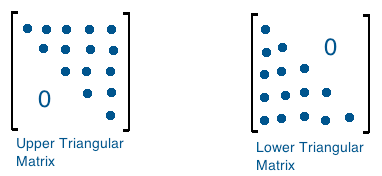
\includegraphics[width=0.42\columnwidth]{UpperLowerTriangularImage.png}}%
% \caption[]{To be described}% \squeezeup
% \vspace{-2mm}
% \end{figure}
 
%  \textbf{Remark:} In HW you will develop Julia code to solve triangular systems of equations, whether upper or lower triangular. Your data will be given to you sometimes as systems of equations written out as formulas and sometimes directly as matrices. We'll also have you upload some BIG matrices and give it a go! 
 
 \section{A Simple Trick with Systems of Equations: Re-arranging their Order}
 \label{sec:SwappingRows}
 
This system of equations is neither upper triangular nor lower triangular
\begin{equation}
\label{eq:BeforeSwapping0}
    \begin{aligned}
     3 x_1 &=6 \\
    x_1 - 2 x_2 + 3 x_3  &= 2 \\
         2 x_1 - x_2 &= -2.
    \end{aligned}
\end{equation}
We can simply re-arrange the order of the equations to arrive at
\begin{equation}
\label{eq:AfterSwapping0}
    \begin{aligned}
     3 x_1 &=6 \\
         2 x_1 - x_2 &= -2 \\
             x_1 - 2 x_2 + 3 x_3  &= 2 ,
    \end{aligned}
\end{equation}
which happens to be lower triangular. We still have the same equations and hence their solution has not changed. The equations have just been re-arranged to make the process of computing their solution fall into a nice pattern that we already know how to handle.
\begin{tcolorbox}
\textbf{This is a really useful trick in mathematics: re-arranging a set of equations without changing the answer.} Right here, it may seem kind of trivial, but when we look at this in terms of matrices in the next Chapter, we get a cool piece of insight. 
\end{tcolorbox}




\section{Looking Ahead}

Once again, our goal is to solve very large sets of linear equations, say more than 100 variables. In this chapter, we saw how to solve problems with triangular structure. Our next major way point is to reduce all linear systems of $n$-equations in $n$-variables to being solvable with forward substitution and back substitution. To get there we need to understand:
\begin{itemize}
\item the standard way to multiply two matrices
\item a little known way to multiply two matrices
    \item how to \textit{factor} a square matrix as the product of two triangular matrices
\end{itemize}

 \vspace*{.5cm}
\begin{tcolorbox}[title={\large \textcolor{red}{\bf  Help! Help! } \textbf{ How am I supposed to remember all of this?}}]
 
\textbf{ You probably can't. In any case, we don't want you to memorize the ROB 101 material.} Instead, open up a \texttt{google doc or google sheet} and make notes! You need an organized method for keeping track of stuff. In High School, you may have been able to remember all the new notation without any special effort. In College, it's a bit different.
 
 \end{tcolorbox}